\chapter{Physics Objects}
\label{sec:reco}
\section{Introduction}
In the previous chapter, details of the \ac{CMS} detector were presented. We
shall now begin to discuss the algorithms used to reconstruct analysis level
objects and quantities which will be of fundamental importance in later
chapters. The objects of primary interest for these purposes are leptons, jets
and missing energy. The offline reconstruction algorithms used to reconstruct
each object will be presented, along with issues and properties related to data
analysis. Some details of the reconstruction performance at \ac{CMS} will also
be shown. Finally, the \acf{PF} algorithm, which provides a global
reconstruction of the event, will be explained in some detail. As will be seen,
\ac{PF} combines tracking and calorimeter measurements to provide excellent
reconstruction of jets and missing energy.

\section{Leptons}
The reconstruction of charged leptons at \ac{CMS} will now be described. Since
tau leptons are not used by either of the analyses presented in this work, their
reconstruction will not be described here. The interested reader is directed to
relevant literature~\cite{cms_pf_tau_id,tau_reco_cms}.

\subsection{Muons}
\label{sec:reco_muons}
The full details of muon reconstruction at CMS are presented
in~\cite{cms_mu_reco,cms_mu_pas}. A brief overview will be presented here,
focussing on the aspects pertinent to the following analysis chapters. Muons are
reconstructed in both the muon chambers and the silicon tracker. To match this
redundancy in the measurement, a number of reconstruction algorithms are
available.

\subsubsection{Tracker Muons}
Tracker muons begin as tracks in the silicon tracker. All tracks with a $\Pt >
\unit{0.5}{\GeV}$ and $p > \unit{2.5}{\GeV}$ are considered as muon candidates
and extrapolated to the muon stations, accounting for expected energy loss and
multiple scattering effects. If at least one muon track segment matches the
extrapolated tracker track, a tracker muon is reconstructed. This algorithm is
more efficient at low momentum ($p < \unit{5}{\GeV}$) since it requires only a
single segment in the muon chambers.

\subsubsection{Standalone Muons}
Standalone muons are based solely on measurements in the muon chambers. The hits
in each chamber are fit individually to obtain seeds - a position and direction
vector along with an estimate of the transverse momentum. These form the basis
of a track fit in the muon chambers based on the Kalman-filter technique. The
fit is constrained to the vertex in order to reject cosmic ray muons. Since much
of the calibration and validation work for the muon system was performed using
cosmic rays, a separate algorithm was developed for this purpose~\cite{cms_mu_reco_cosmic}.

\subsubsection{Global Muons}
Global muons are an extension of standalone muons to include measurements in the
silicon tracker. For muons with a transverse momentum below $\approx$
\unit{200}{\GeV}, the tracker provides a better momentum resolution. For higher
momentum muons, the tracks become straighter and the momentum measurement
increasingly affected by uncertainty in the position measurement. In this
regime, inclusion of hits in the muon chambers effectively benefits from the
large lever arm and \unit{3.8}{\tesla} magnetic field in the region between the
silicon tracker and the muon chambers.

For each standalone muon, the set of tracker tracks is searched and the best
matching candidate selected. For each pairing found in this way, a Kalman-filter
fit is again performed, this time using hits from both the silicon tracker and
the muon chambers. This fit accounts for average expected energy losses,
magnetic field and multiple scattering effects. The tracks reconstructed by this
procedure are known as global muons. Once again, certain modifications are
required for reconstructing cosmic ray muons - for instance in the case that
cosmic muons traverse the entire detector, leaving two standalone muons on
either side of \ac{CMS}.

\subsubsection{Merging}
Reconstructed muons from each of the algorithms detailed above are then merged
into a single list of muon candidates. Candidates reconstructed as both global
and tracker muons are merged. Standalone muon tracks are merged with tracker
muons if they share a muon segment. The fit results from each algorithm are
retained.

An analysis is then able to tune its identification cuts to meet certain
efficiency or purity requirements for a particular kinematic range. A number1 of
pre-defined selections are available:
\begin{itemize}
\item Soft muons are required to be reconstructed as tracker muons with a muon
  segment in the outermost station matching the position and direction expected
  from extrapolation of the track.
\item Global muon's only requirement is that they be reconstructed as a global
  muon in the sense described above.
\item Tight muons must be reconstructed as both a global muon and a tracker muon
  with a series of additional requirements: a $\Pt > \unit{3}{\GeV}$, a global
  muon track fit with a normalised $\chisq < 10$, at least two muon stations
  with matching muon segments, at least 10 hits in the silicon tracker (with at
  least 1 pixel hit) and a transverse impact parameter $\dxy <
  \unit{2}{\milli\metre}$. This selection significantly suppresses
  decays-in-flight at the cost of a small loss in efficiency for prompt muons.
\end{itemize}


\subsection{Electrons}
\label{sec:reco_electrons}
Electron reconstruction at \ac{CMS} makes use of measurements from both the
silicon tracker and the \ac{ECAL}. In the case of \ac{CMS}, the large amount of
material in the tracker causes electrons to radiate a large fraction of their
energy before reaching the \ac{ECAL} - 50\% of electrons radiate more than 50\%
of their energy in this way. For an accurate measurement of the electron energy,
this energy, radiated in the form of bremsstrahlung photons, must be
reconstructed correctly.

\subsubsection{Reconstruction}
Electron seeds are derived using two separate algorithms: \emph{tracker-driven}
and \emph{\ac{ECAL}-driven}~\cite{cms_ele_reco}. The tracker-driven algorithm was
developed for the purposes of the \ac{PF} algorithm. It is most suitable for
low-\Pt electrons and electrons produced inside jets. Seeds are found by
extrapolating \ac{GSF} tracks in the tracker from their outermost measurement to
the \ac{ECAL}. If a matching cluster is found, a tracker-driven seed is
created~\cite{cms_pf_pas3}.

\ac{ECAL}-driven seeds begin with the reconstruction of \ac{ECAL} superclusters
with transverse energy, $\Et > \unit{4}{\GeV}$. A supercluster is a group of one
or more \ac{ECAL} clusters constructed to account for the narrow $\eta$ width
and spread in $\phi$ due to the bending effect of the \ac{CMS} magnet on
electrons radiating in the tracker~\cite{cms_ele_reco_pas}. These superclusters
are then matched to track seeds with two or three hits in the inner layers of
the tracker. Electron tracks are built from these track seeds. Trajectories are
calculated accounting for energy loss in the tracker. These are then fit with a
\ac{GSF}~\cite{gsf}.

Candidates found only by the tracker-driven method must pass a pre-selection
based on a multivariate analysis~\cite{cms_pf_pas3}. Candidates found by the
\ac{ECAL}-driven algorithm are pre-selected by matching the \ac{GSF} track to
the supercluster in $\eta$ and $\phi$. \ac{ECAL}-driven seeds failing this
matching requirement, but selected by the track-driven multivariate
pre-selection are kept.

As described in Section~\ref{sec:expt_laser_monitoring}, electron energies are
corrected to account for changes in the transparency of the \ac{ECAL}
crystals. For the \PW polarisation measurement, a set of ``ad-hoc'' corrections
were calculated from fits to the \PZ mass. For the \ac{SUSY} search analysis,
more sophisticated corrections were available~\cite{laser_monitoring}.

\subsubsection{Electron Identification}
\label{sec:reco_electron_id}
The large bremsstrahlung induced energy loss coupled with larger backgrounds
from jets and photons means that electrons at \ac{CMS} are fundamentally less
well defined object than muons. There is therefore a much larger space to
trade-off between signal efficiency and purity. Whilst more complex selection
procedures are available (e.g. a multivariate approach), a simple cut-based
selection was chosen for the \PW cross-section
measurement~\cite{cms_pas_ewk_10_002, simple_eleid_web} and has been used in this work. The
variables have been chosen for their background rejection capabilities but also
for robustness during early the data-taking period. Cut values have been chosen
for a number of working points, defined by their efficiency with respect to a
simulated \Wenu sample, and optimising the background rejection power using an
iterative procedure. Different cut values are chosen in the \ac{CMS} barrel and
endcap regions.

The cut variables used are described below, with cut-values for each working
point shown in Table~\ref{tbl:reco_electronid}
\begin{itemize}
\item \sigmaieta is a measure of the \ac{RMS} shower width of the electron
  in the $\eta$ direction.
\item \deltaphiin and \deltaetain represent the angular separation between the
  trajectory of the \ac{GSF} track and the \ac{ECAL} supercluster.
\item Tracker, \ac{ECAL} and \ac{HCAL} isolation quantities summed in a cone
  $\Delta R < 0.3$~\cite{lepton_isolation_an}. The energy deposits and track
  associated with the lepton are removed. Within the tracker, a threshold of
  \unit{700}{\MeV} is applied to the tracks contributing to the sum. Similarly,
  in the \ac{ECAL}, a zero-suppression cut is applied (\unit{0.08}{\GeV} in
  \ac{EB} and \unit{0.1}{\GeV} in \ac{EE}). The cone is centred on the track
  direction at the vertex for the tracker isolation, and the supercluster for
  the calorimeter quantities. The combined isolation, \CombIso, is then defined
  as
  \begin{equation*}
    \CombIso = \frac{\sum_{\textrm{tracks}} p_T^{\textrm{track}} + \sum_{\textrm{dep}}
    E_T^{\textrm{em}} + \sum_{\textrm{dep}} E_T^{\textrm{had}}}{\Pte}
   \end{equation*}
   where the sums run over the aforementioned tracks, \ac{ECAL} energy deposits
   and \ac{HCAL} energy deposits.
\item \HoverE is the ratio of the energy deposited in the \ac{HCAL} behind the
  electron seed to that in the \ac{ECAL}. This might also be called the
  \ac{HCAL} leakage.
\end{itemize}

The remaining variables are chosen to reject electrons stemming from converted
photons~\cite{cms_an_2009_159}. For conversions which occur after the first
layer of the tracker, these may exhibit a pattern of \emph{missing hits} -
i.e. layers of the inner tracker without a hit where one would be expected from
extrapolation of the track. Conversions can be rejected by requiring either no
such missing hits, or a single missing hit depending on the desired efficiency.

\begin{itemize}
\item Further rejection against electron conversions is provided by the
  variables \Distnm and \DeltaCotThetanm. Firstly, potential conversion partners
  are found by pre-selecting all \ac{CTF} fitted tracks in a cone $\DeltaR <
  0.3$ of the \ac{GSF} track, and having opposite charge. For each of these,
  \DeltaCotThetanm is calculated as
\begin{equation*}
  \DeltaCotThetanm = \cot\left(\Theta_{\textrm{CTF track}}\right) - \cot\left(\Theta_{\textrm{GSF track}}\right)
\end{equation*}
\item \Distnm is defined as the two-dimensional distance in the $x-y$ plane between the
two tracks at the point at which they would be parallel when extrapolated. The
choice of \ac{CTF} tracks is restricted to avoid picking the track corresponding
to the electron. Conversion electrons will tend to have smaller values of
\DeltaCotTheta and \Dist. If a suitable partner track is found, the electron is
rejected if both \Dist and \DeltaCotTheta are below given thresholds.
\end{itemize}

The pseudorapidity acceptance for electrons is $|\eta| < 2.5$. However, the
barrel-endcap transition region, $1.4442 < |\eta| < 1.566$ is explicitly excluded.

\ctable[
caption=Table showing cut values for the simple cut-based electron indentification working points,
label=tbl:reco_electronid
]{lcccccc}{
}{\FL
Efficiency           & 0.95  & 0.9   & 0.85  & 0.8   & 0.7   & 0.6 \ML
\multicolumn{7}{c}{Conversion Rejection}\ML
Missing Hits         & 1     & 1     & 1     & 0     & 0     & 0 \NN
\Dist                & -     & 0.02  & 0.02  & 0.02  & 0.02  & 0.02\NN
\DeltaCotTheta       & -     & 0.02  & 0.02  & 0.02  & 0.02  & 0.02\ML
\multicolumn{7}{c}{Barrel}\ML
Combined Isolation   & 0.15  & 0.1   & 0.09  & 0.07  & 0.04  & 0.03 \NN
\sigmaieta           & 0.01  & 0.01  & 0.01  & 0.01  & 0.01  & 0.01 \NN
\deltaphiin          & 0.8   & 0.8   & 0.06  & 0.06  & 0.03  & 0.025 \NN
\deltaetain          & 0.007 & 0.007 & 0.006 & 0.004 & 0.004 & 0.004 \NN
\HoverE              & 0.15  & 0.12  & 0.04  & 0.04  & 0.025 & 0.025 \ML
\multicolumn{7}{c}{Endcaps}\ML
Combined Isolation   & 0.1   & 0.07  & 0.06  & 0.06  & 0.03  & 0.02 \NN
\sigmaieta           & 0.03  & 0.03  & 0.03  & 0.03  & 0.03  & 0.03 \NN
\deltaphiin          & 0.7   & 0.7   & 0.04  & 0.03  & 0.02  & 0.02 \NN
\deltaetain          & 0.01  & 0.009 & 0.007 & 0.007 & 0.005 & 0.005 \NN
\HoverE              & 0.07  & 0.05  & 0.025 & 0.025 & 0.025 & 0.025 \LL
}

\section{Jets}
\label{sec:reco_jets}
Four types of jets are reconstructed at \ac{CMS}: \acf{Calo} jets, \ac{PF} jets,
\ac{JPT} jets and track jets~\cite{jet_perf_pas}. \ac{Calo} jets are
reconstructed from energy deposits in the \ac{ECAL} and \ac{HCAL}, combined into
calorimeter towers. Calorimeter towers consist of one or more \ac{HCAL} cells
with geometrically matched \ac{ECAL} crystals. The exact details of this
association varies between the barrel and endcap regions. Electronics noise is
suppressed by applying a threshold to calorimeter cells, with pile-up effects
reduced by a requirement on the tower energy.

\ac{JPT} jets associate tracks with \ac{Calo} jets, using the tracker to give
enhanced \Pt resolution and response. \ac{PF} jets are products of the \acl{PF}
algorithm described below. Finally, track jets are reconstructed from well
measured tracks in the central tracker. Jets are clustered using the \antiKT
algorithm~\cite{antiKT} with a size parameter $R=0.5$.

\subsection{Jet Energy Corrections and \acl{JES}}
Since the jet energy as measured by the detector is generally different from the
corresponding particle jet energy, jet energy corrections are
applied~\cite{jet_energy_cms, jet_energy_pas}. At \ac{CMS}, these have been been
factorised into three parts:
\begin{itemize}
\item \emph{offset corrections} remove excess energy from electronics noise and
  pile-up;
\item \emph{relative corrections} attempt to remove variations in jet response
  with respect to pseudorapidity
\item \emph{absolute corrections} attempt to remove variations in jet response
  with respect to \Pt.
\end{itemize}
These are measured using a variety of techniques including the balancing of
dijets, \gammajets and \Zjets events. Figures~\ref{fig:reco_jet_energy_corr}
show these correction factors as a function of $\eta$ for two values of the jet
\Pt. With these corrections applied, the residual uncertainty on the \ac{JES}
has been evaluated as a function of jet $\eta$ and \Pt. This will turn out to be
a dominant source of systematic uncertainty for the analyses presented here.

\begin{figure}
  \centering
  \subfloat[\unit{50}{\GeV}]{\label{fig:jet_energy_corr_50}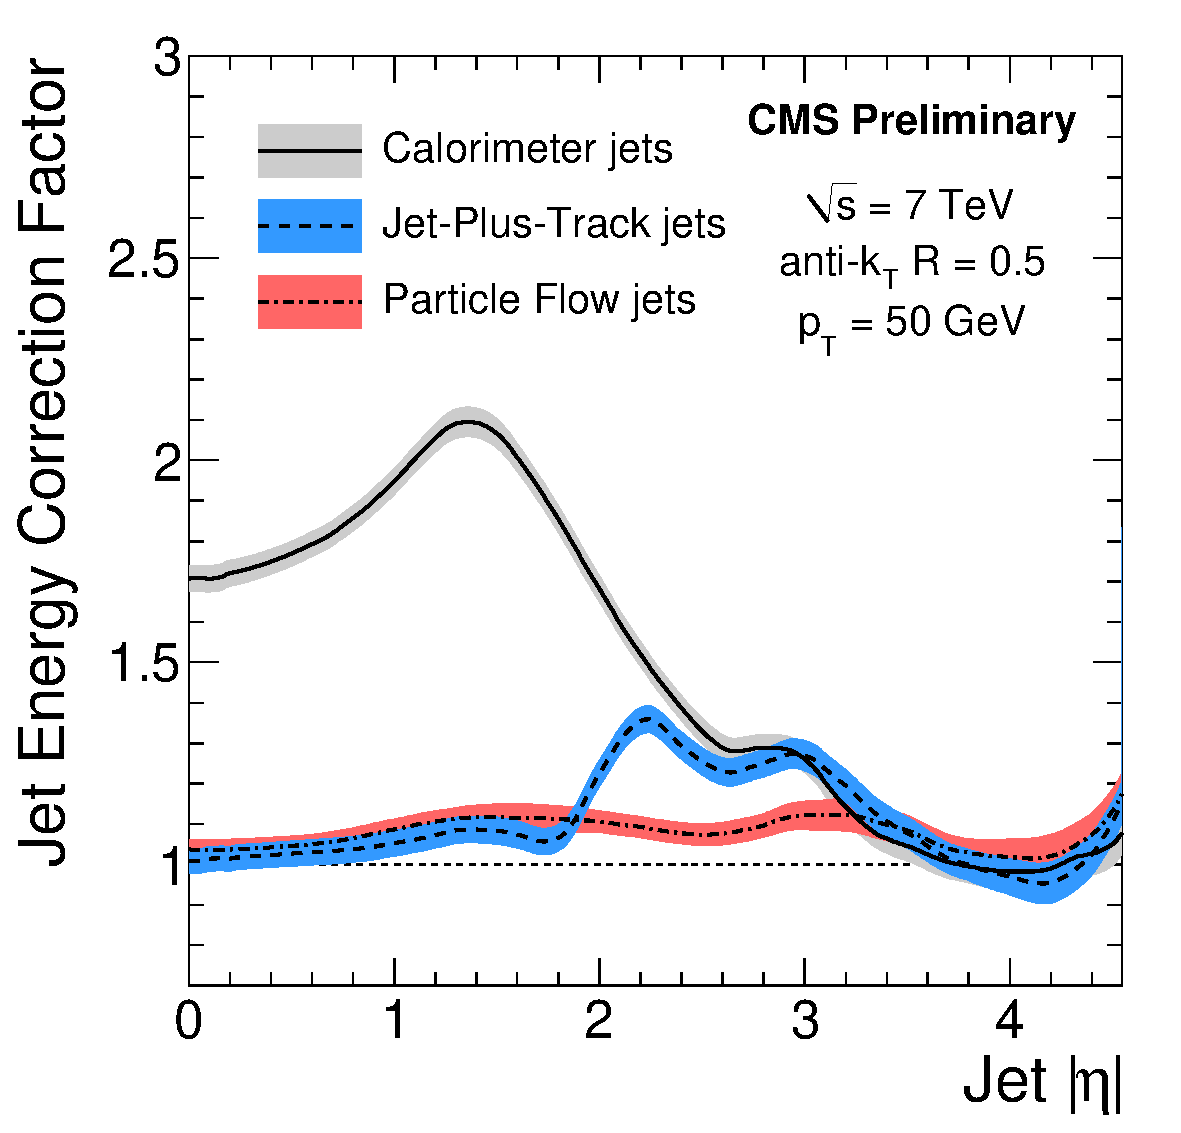
\includegraphics[width=0.45\textwidth]{fig/jet_energy_corr_pt50.pdf}}\quad
  \subfloat[\unit{200}{\GeV}]{\label{fig:jet_energy_corr_200}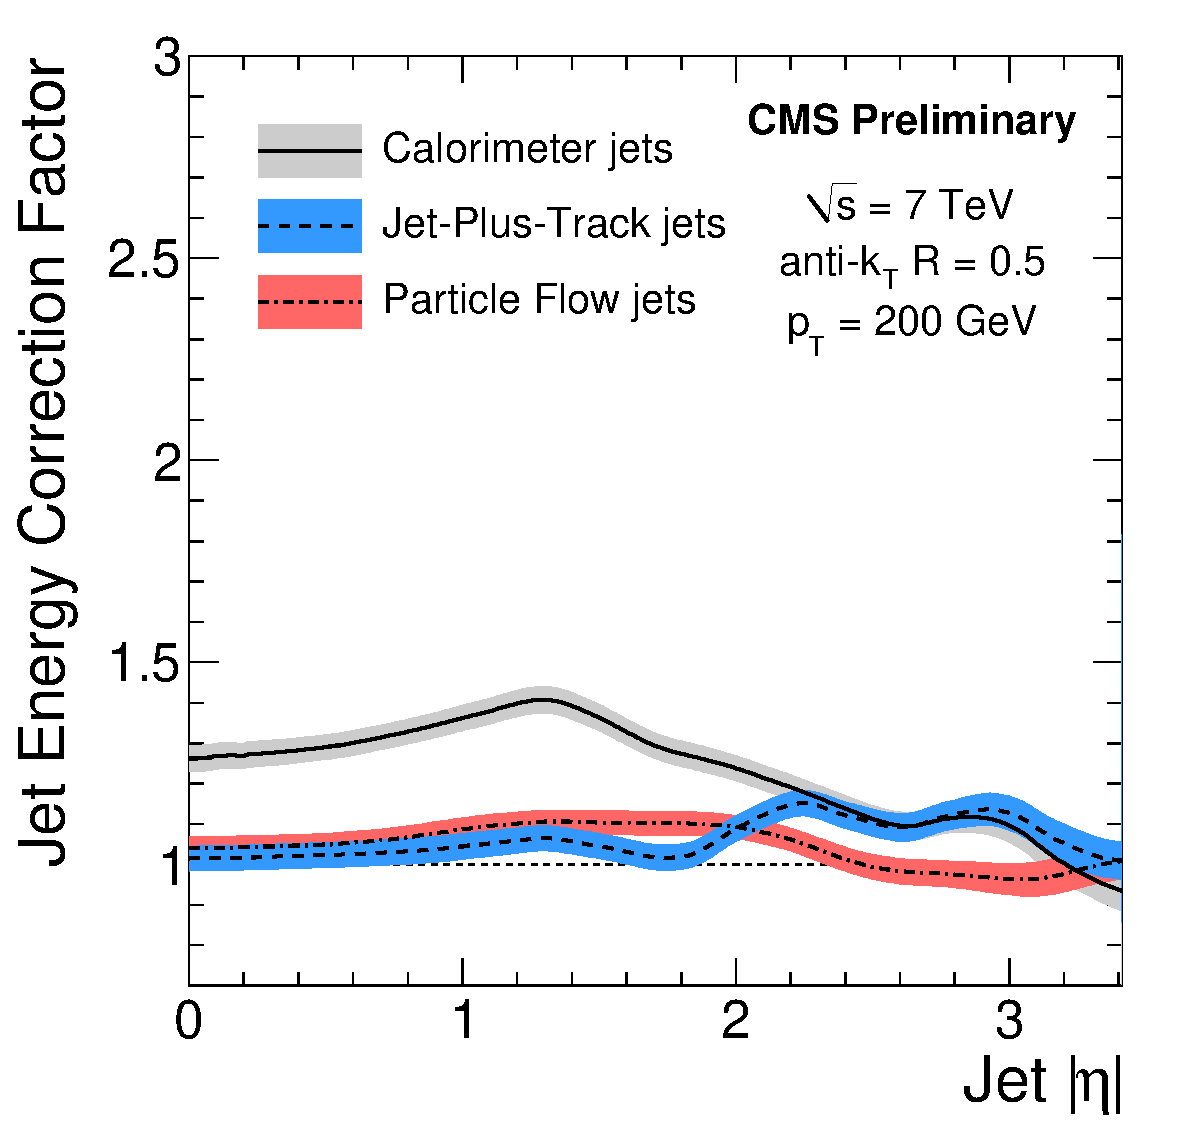
\includegraphics[width=0.45\textwidth]{fig/jet_energy_corr_pt200.pdf}}\quad
  \caption[Total jet energy correction factor as a function of $\eta$ for jets
  with transverse momenta of \unit{50}{\GeV} and \unit{200}{\GeV}]{Total jet
    energy correction factor as a function of $\eta$ for jets with transverse
    momenta of \unit{50}{\GeV} and \unit{200}{\GeV}. Corrections are shown for
    \ac{Calo}, \ac{JPT} and \ac{PF} jets separately. The bands indicate the
    corresponding uncertainties~\cite{jet_energy_pas}.}
  \label{fig:reco_jet_energy_corr}
\end{figure}

\section{Missing Energy}
Certain particles, such as neutrinos, are not reconstructed by the \ac{CMS}
detector. However, their presence may be inferred by considering the total
momentum of particles reconstructed by the detector and comparing this with the
momentum of the initial state. Any imbalance in these quantities can be
attributed to the presence of some ``invisible'' particles - a \emph{missing
  energy} signature.

At a hadron collider, the situation is complicated by the fact that the boost of
the initial partons parallel to the beamline is not known. Hence missing energy
measurement along this axis is not possible. For this reason, transverse
quantities are used instead - most commonly the \emph{missing transverse
  energy}, \METv. This can be defined generically as
\begin{equation*}
\METv = -\sum_{o in \textrm{objects}} \vec{p}_T^o
\end{equation*}
where $p_T^o$ refers to the transverse momentum of object $o$. The chosen set of
objects then leads to a number of alternative definitions of \METv. The
magnitude of this quantity, often used in event selection, will be denoted
\MET. Similar notation will be used for other transverse vector quantities.

At \ac{CMS}, the simplest measurement of \METv is \ac{Calo} \METv which sums
over the calorimeter tower energies (\ac{ECAL} and \ac{HCAL}).  An energy
threshold is applied to the towers in order to reject electronics
noise. Alternatively, \ac{PF} \METv sums over the candidate particles output by
the \ac{PF} algorithm. This will be discussed further in
Section~\ref{sec:reco_pf}. As will be seen, this provides the most sensitive
\METv measurement at \ac{CMS} and thus is used throughout the work presented
here. It should be assumed, unless noted otherwise, that references to \METv or
derived quantities use the \ac{PF} measurement.

Alternative missing energy quantities can be defined for other purposes. Often,
a scalar quantity is desired instead. The \emph{missing transverse hadronic
  energy} (\MHT) is formed by taking the vector sum,
\begin{equation}
\MHTv = -\sum_{j \in \textrm{jets}} \vec{E_T^j}
\end{equation}
In general, this is used to measure the energy of a system of particles
recoiling against the jets in an event. For example, in \Wjets events, the
recoiling system is the \PW boson. \MHTv is therefore one possible measurement
of the \PW boson transverse momentum, \PtWv.


\section{Particle Flow at \ac{CMS}}
\label{sec:reco_pf}
The \ac{PF} algorithm~\cite{cms_pf_pas, cms_pf_pas2} attempts to provide a
global reconstruction of the event - accurate determination of the type, energy
and direction of all stable particles - by combining measurements from all
subdetectors in \ac{CMS}. This strategy is well suited for use with the \ac{CMS}
detector. The silicon tracker is able to reconstruct charged particle tracks
with high efficiency and purity down to transverse momenta as low as
\unit{150}{\MeV}. Additionally, the granularity of the \ac{ECAL} is sufficient
for the separation of photons and charged particle energy deposits in jets with
\Pt of a few hundred \GeV~\cite{cms_pf_pas}. In contrast, the \ac{HCAL} is much
coarser. However, the combined energy resolution of both calorimeters is $\sim
10\%$ at \unit{100}{\GeV}. This allows identification of the energy deposits
associated with neutral hadrons as an excess on top of that accounted for by
matching the deposits with charged tracks. The \ac{PF} algorithm is able to
reconstruct the components of jets and hadronic tau decays - primarily charged
hadrons, neutral hadrons and photons. This provides an improved measurement of
the jet energy and thus also of \METv.

The particle flow algorithm proceeds by linking the tracks and energy clusters
to form blocks. A typical event display illustrating this process is shown in
Figure~\ref{fig:reco_pf_diag}. A single block may contain some combination of a
charged particle track, one or more energy clusters and a muon. The fine
granularity of the \ac{CMS} detector ensures that blocks typically contain 1, 2
or 3 elements.  The links between each block are parameterised by a distance
which encodes the quality of the link. Advanced tracking and calorimeter
clustering algorithms have been developed to meet the needs of the \ac{PF}
algorithm. These will now be explained.

\begin{figure}[h!]
\centering
\subfloat[]{\label{fig:reco_pf_diag1}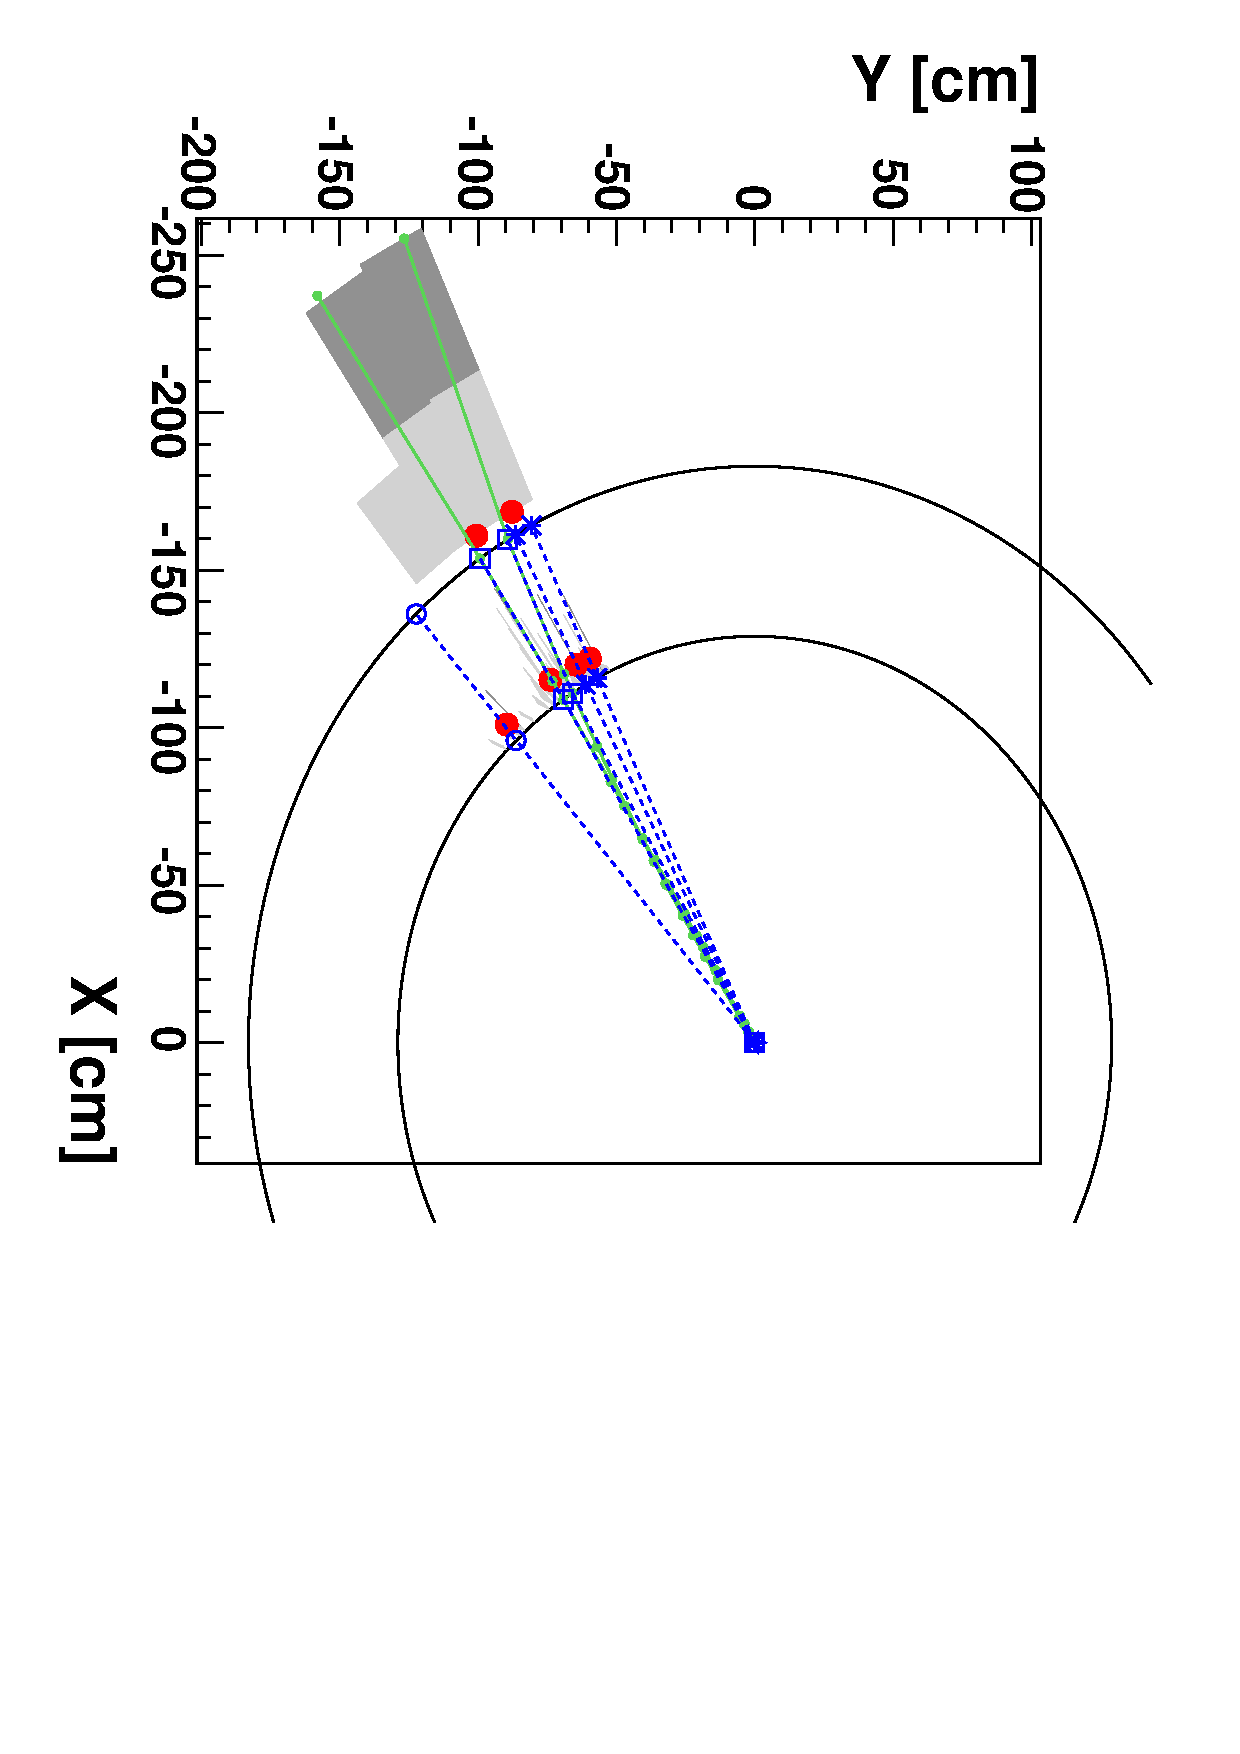
\includegraphics[width=0.7\textwidth]{fig/pf_diag1}}\\
\subfloat[]{\label{fig:reco_pf_diag2}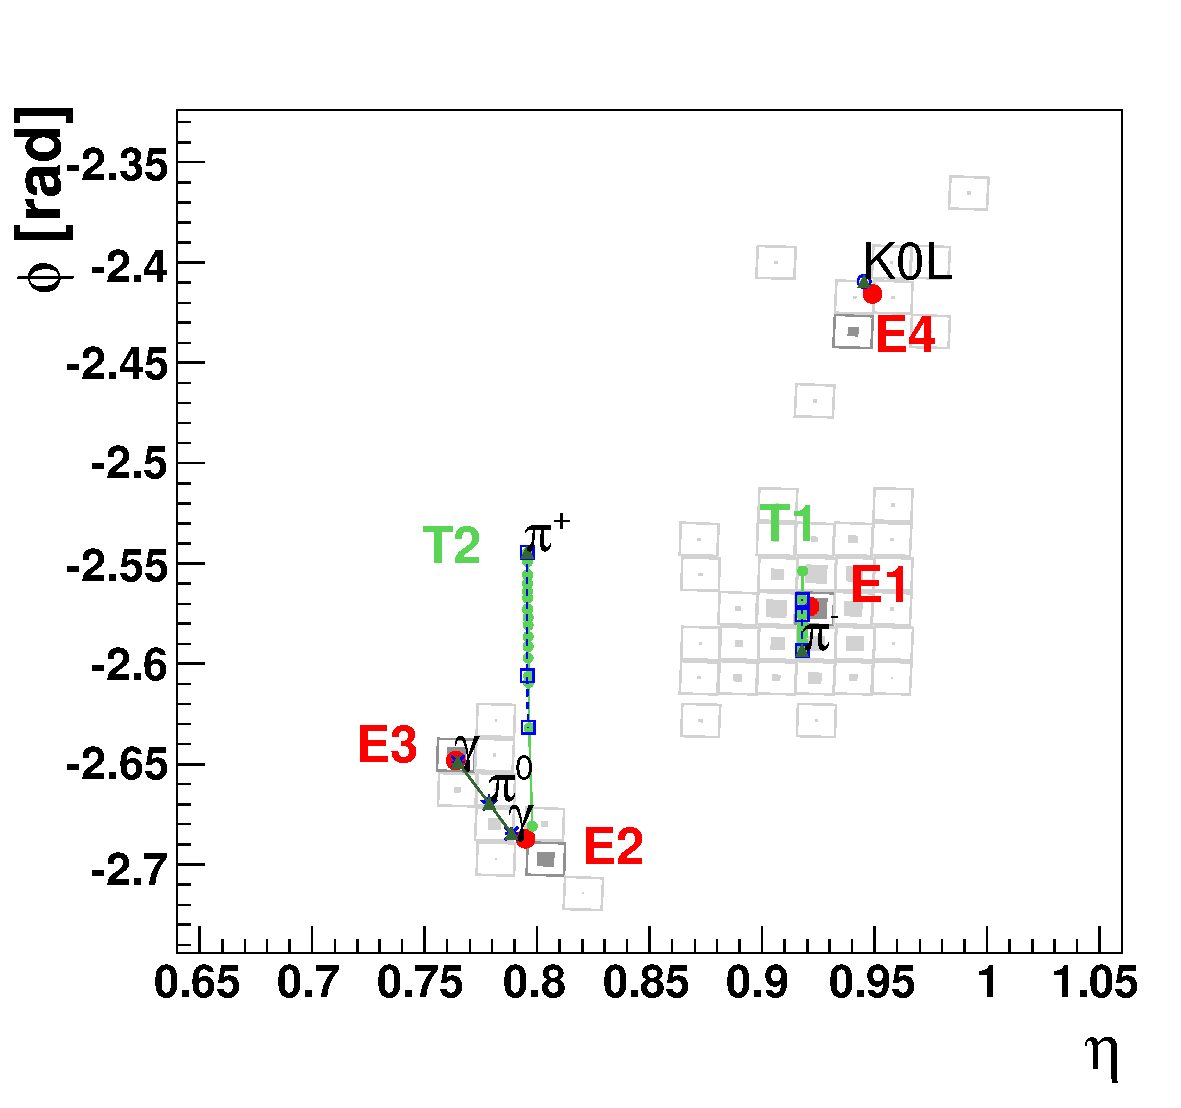
\includegraphics[width=0.45\textwidth]{fig/pf_diag2}}\quad
\subfloat[]{\label{fig:reco_pf_diag3}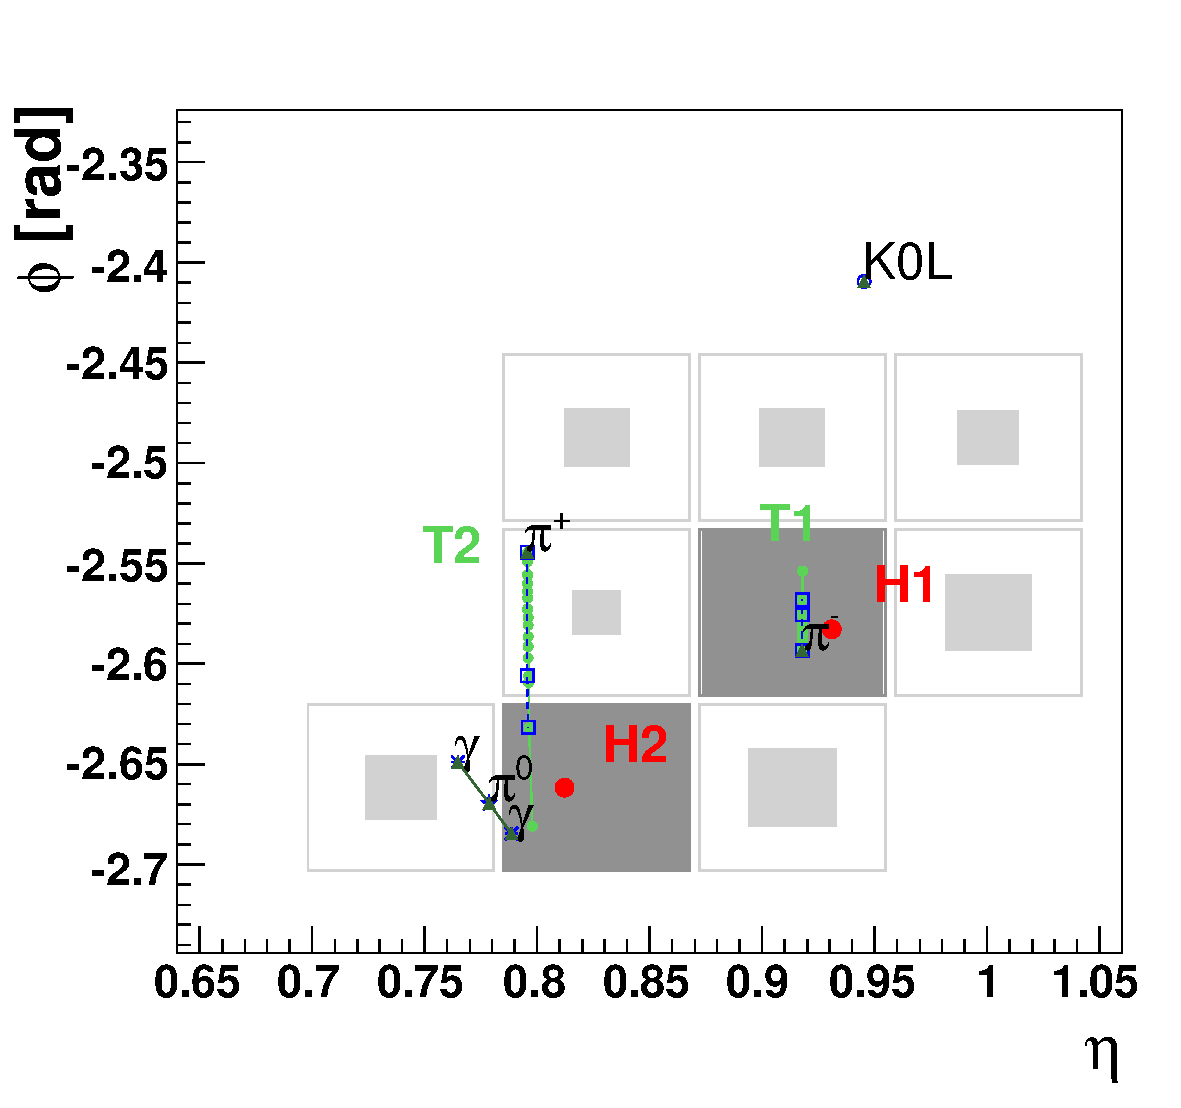
\includegraphics[width=0.45\textwidth]{fig/pf_diag3}}
\caption[]{An event display showing a hadronic jet in~\subref{fig:reco_pf_diag1}
  the $(x,y)$-plane, \subref{fig:reco_pf_diag2} an $(\eta,\phi)$ view at the
  surface of the \ac{ECAL} and~\subref{fig:reco_pf_diag3} the same orientation
  at the surface of the \ac{HCAL}. These two surfaces appear as circular arcs
  in~\subref{fig:reco_pf_diag1}. The \PKlong, \Ppiminus, \Ppiplus, \Ppizero and
  the two photons from its decay are shown. The \PKlong, \Ppim and two photons
  result in clear, well-speparated \ac{ECAL} cluters - round points labelled E1
  to E4~\ref{fig:reco_pf_diag2}. The \Ppiplus and \Ppiminus are reconstructed
  as charged tracks - green lines labelled T1 and T2 - which point to the two
  \ac{HCAL} clusters - round points labelled H1 and H2.}
\label{fig:reco_pf_diag}
\end{figure}

\subsection{Iterative Tracking}
The measurements of momentum and direction of charged hadrons provided by the
tracker are hugely superior to those that can be provided by the calorimeters.
It is important therefore that the tracks input to the \ac{PF} procedure be
reconstructed with near 100\% efficiency. The fake rate must also be low to
avoid excess energy counting.

To meet these requirements, tracks are reconstructed using an iterative
algorithm. This begins by reconstructing tracks with very tight selection
requirements. Hits which can be unambiguously assigned in this step are then
removed from consideration. The algorithm is iterated, attempting to reconstruct
tracks from the remaining hits, this time with loosened selection criteria. This
procedure is repeated with progressively looser selection criteria. This ensures
high efficiency, whilst the removal of hits at each stage reduces the fake rate
induced by combinatorics.  After three iterations, tracks originating close to
the beam line are reconstructed with an efficiency of 99.5\% for muons and
$>90\%$ for charged hadrons. The fourth and fifth iterations relax constrains on
the vertex, reconstructing secondary charged particles.

\subsection{Calorimeter Clustering}
The success of the \ac{PF} reconstruction is dependent on certain aspects of the
clustering algorithm. In particular, as for the tracks, the clustering needs to
be highly efficient and be able to distinguish closely spaced energy deposits.
To this end, a specialised clustering algorithm was developed. This algorithm is
used the \ac{ECAL}, \ac{HCAL}, \ac{PS} but not in the \ac{HF} where each cell is
taken to be a cluster.

The first step of the algorithm produces \emph{seed clusters} from local maxima
in the calorimeter cell energies meeting a minimum threshold requirement.  These
seed clusters are then extended to include cells sharing at least one side in
common with the original cluster and an energy exceeding a threshold chosen
according to the standard deviation of electronics noise in the
calorimeter. These \emph{topological clusters} are then transformed into
\emph{particle flow clusters}, with a separate particle flow cluster for each
seed comprising the topological cluster. The energy and position of each
particle flow cluster is determined iteratively, with the energy of each cell
shared among the particle flow clusters.

\subsection{Building Links}
Each track is extrapolated from the position of its last measured hit to the
\ac{PS}, the \ac{ECAL} at a depth corresponding to the expected maximum for an
electron shower, the \ac{HCAL} at a depth of 1 interaction length. If the
extrapolated track position lies within the envelope of a cluster, a link is
created with a link distance equal to the $(\eta, \phi)$ distance between the
extrapolated track and the cluster. The envelope may be enlarged with respect to
the cluster by the extent of a single cell.

Additionally, energy contributions from bremsstrahlung photons are included by
extrapolating the track tangent at each tracker layer to the \ac{ECAL}. If the
extrapolated track lies within the envelope of the cluster, a link is created.
Links are also created between calorimeter clusters in different subdetectors if
the cluster position in the finer-grained calorimeter lies within the envelope
of the more coarsely grained calorimeter. The link distance is taken to be the
$(\eta, \phi)$ separation of the two clusters.

Muons are included when a global fit between a track in the tracker and a muon
track in the muon chambers yields an acceptable \chisq. If several global muons
are found for a single muon track, only that possessing the smallest \chisq is
retained - with the link distance determined by the \chisq.

\subsection{Particle Reconstruction}
The first step is to reconstruct muons. Each global muon gives rise to a
particle flow muon providing its momentum as determined from the global fit is
compatible with the track momentum to within 3 standard deviations. The
corresponding track is then removed from the block.

The next step is electron reconstruction. Electron tracks in the block are first
selected by a pre-identification step - electrons often leave short tracks and
lose energy via bremsstrahlung. Pre-identified electrons are then refit with a
Gaussian Sum Filter (see Section~\ref{sec:reco_electrons}) and projected into
the \ac{ECAL}.  Candidates passing tracking and calorimetric criteria are
reconstructed as particle flow electrons. The track and associated \ac{ECAL}
clusters are then removed from the block.

Tracks remaining are then subject to a tighter set of quality requirements, in
particular that the track \Pt uncertainty be smaller than the relative
calorimeter energy resolution for a charged hadron. Whilst some real hadrons are
lost by this requirement, the energy will be retained in the more accurate
measurement of the calorimeter.

Reconstruction of photons and neutral hadrons involves comparison of the track
momentum to the calorimetric energy. The cluster energies in the \ac{ECAL} are
calibrated for photons and the \ac{HCAL} for \unit{50}{\GeV} pions. For the
comparison to be valid, these must be re-calibrated to account for
non-linearities in the \ac{HCAL} as well as the differing response of the
\ac{ECAL} to hadrons.

In the case that several tracks are linked to a single \ac{HCAL} cluster, the
total momenta of the tracks is compared to the calibrated calorimetric energy.
Tracks linked to multiple clusters are resolved by preserving the closest link
or links in certain cases. The track momentum is then compared to the total
calibrated calorimetric energy.

In the rare case that the energy is smaller than the track momentum by more than
three standard deviations, a relaxed search for fake tracks and global muons is
initiated. Global muons are identified as \ac{PF} muons if their momentum is
measured with an uncertainty below 25\%. Tracks are then progressively removed
from the block, those with largest momentum uncertainty first, until either all
tracks with an uncertainty $>\unit{1}{\GeV}$ have been considered or the total
track momentum has decreased below the calorimetric energy. The remaining tracks
are interpreted as charged hadrons with momentum and energy taken from the track
momentum assuming the charged pion mass hypothesis. If the calorimeter energy
and track momentum are compatible within their uncertainties, the momentum is
redefined by a fit to both track momenta and the energy cluster. This is helpful
at very high energies, where the track parameters may be less well measured.

In the case that the calibrated energy is greater than the total track momentum
by more than the calorimetric energy resolution, the excess is interpreted as
a photon and possibly a neutral hadron. If the excess is greater than the
\ac{ECAL} energy, a photon is created with this energy and the rest of the
excess interpreted as a neutral hadron. Otherwise, a photon only is
reconstructed from the uncalibrated \ac{ECAL} energy. This stems from the
observation that photons carry 25\% of the energy of a jet, with neutral hadrons
only 3\%.

Remaining \ac{ECAL} and \ac{HCAL} clusters not linked to a track (or for which
the associated track was disabled in the previous steps) are reconstructed as
photons and neutral hadrons respectively.

\ac{PF} jets are reconstructed by applying the \antikT algorithm to the full set
of \ac{PF} objects.

\subsection{Physics Performance}
Two aspects of the performance of the \ac{PF} reconstruction are of relevance to
the analysis description that will follow: measurement of \METv and jet
reconstruction.

\begin{figure}
\centering
\subfloat[]{\label{fig:reco_pf_jet_energyres_barrel}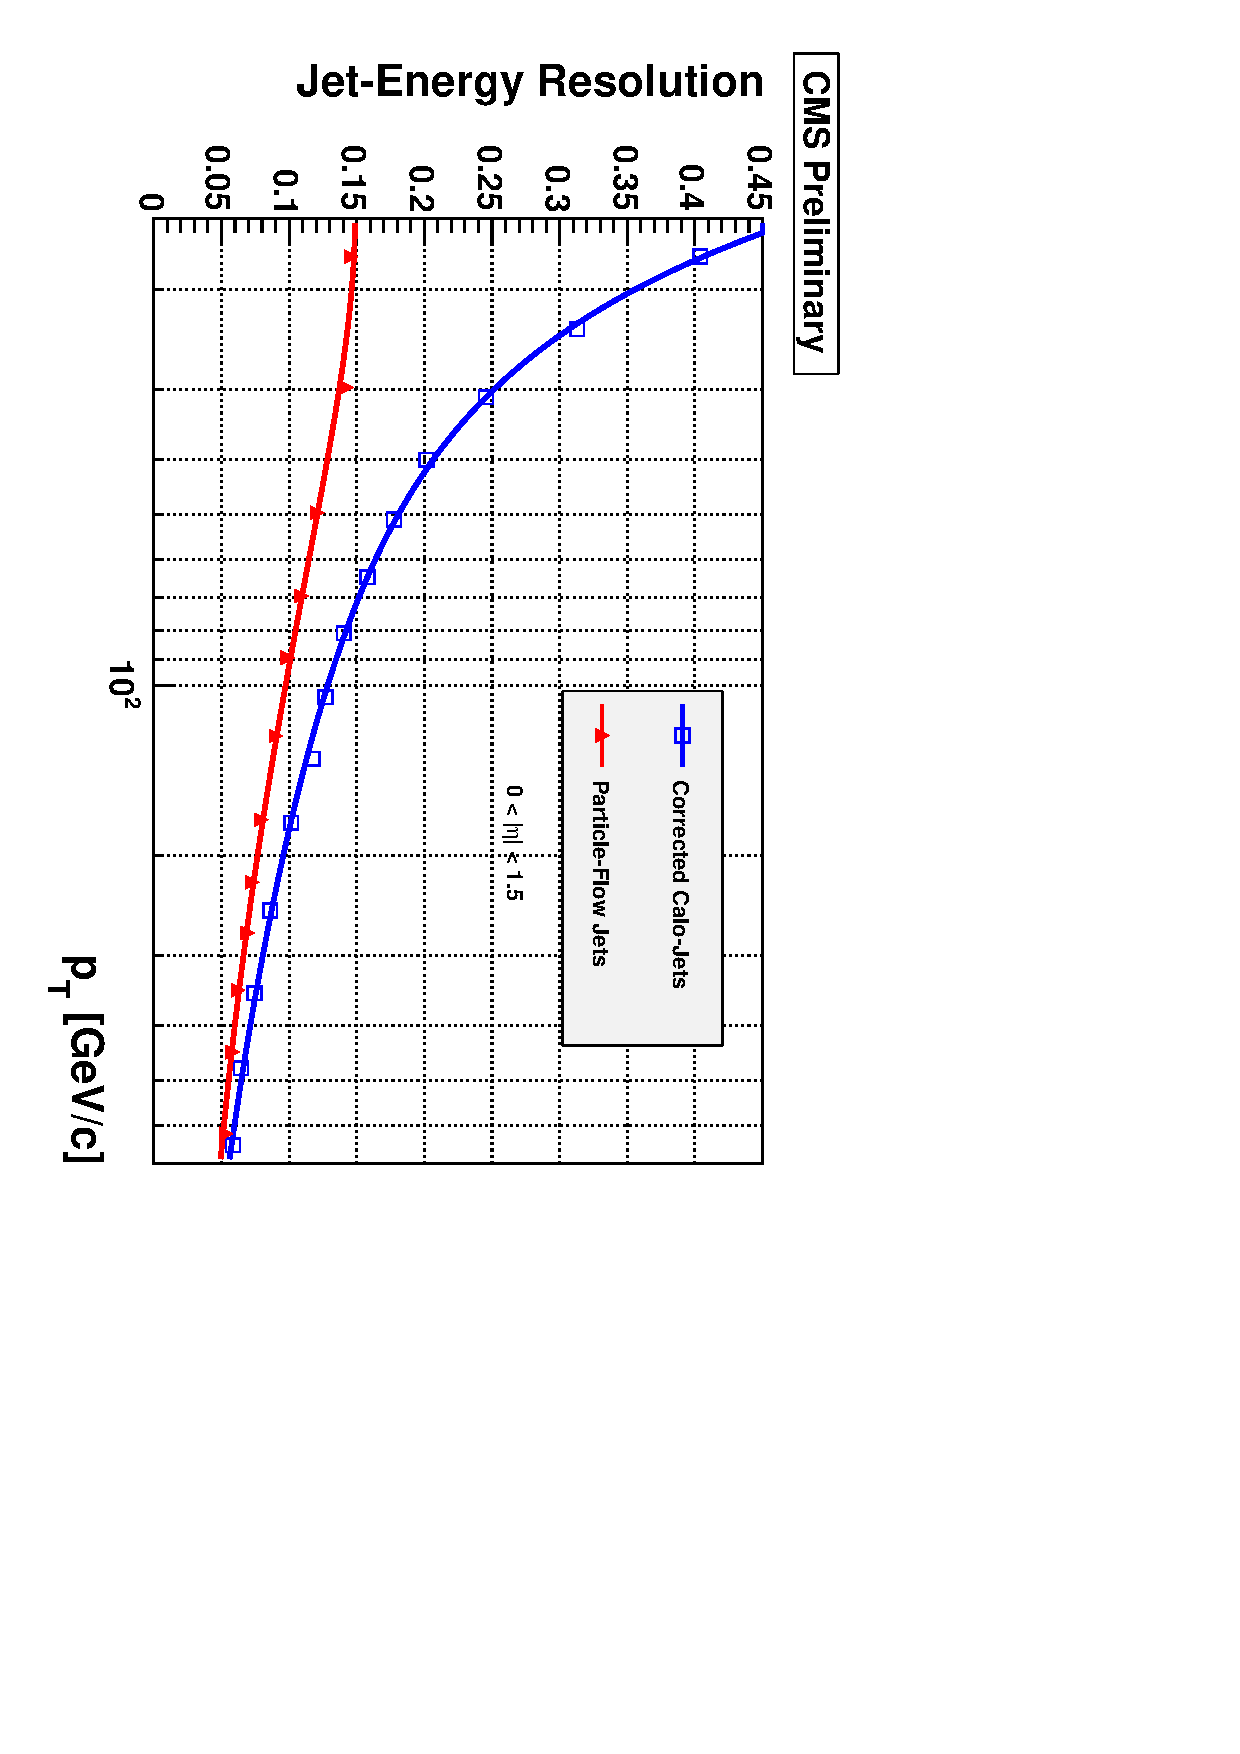
\includegraphics[width=0.45\textwidth]{fig/pf_jet_energyres_barrel}}\quad
\subfloat[]{\label{fig:reco_pf_jet_energyres_endcap}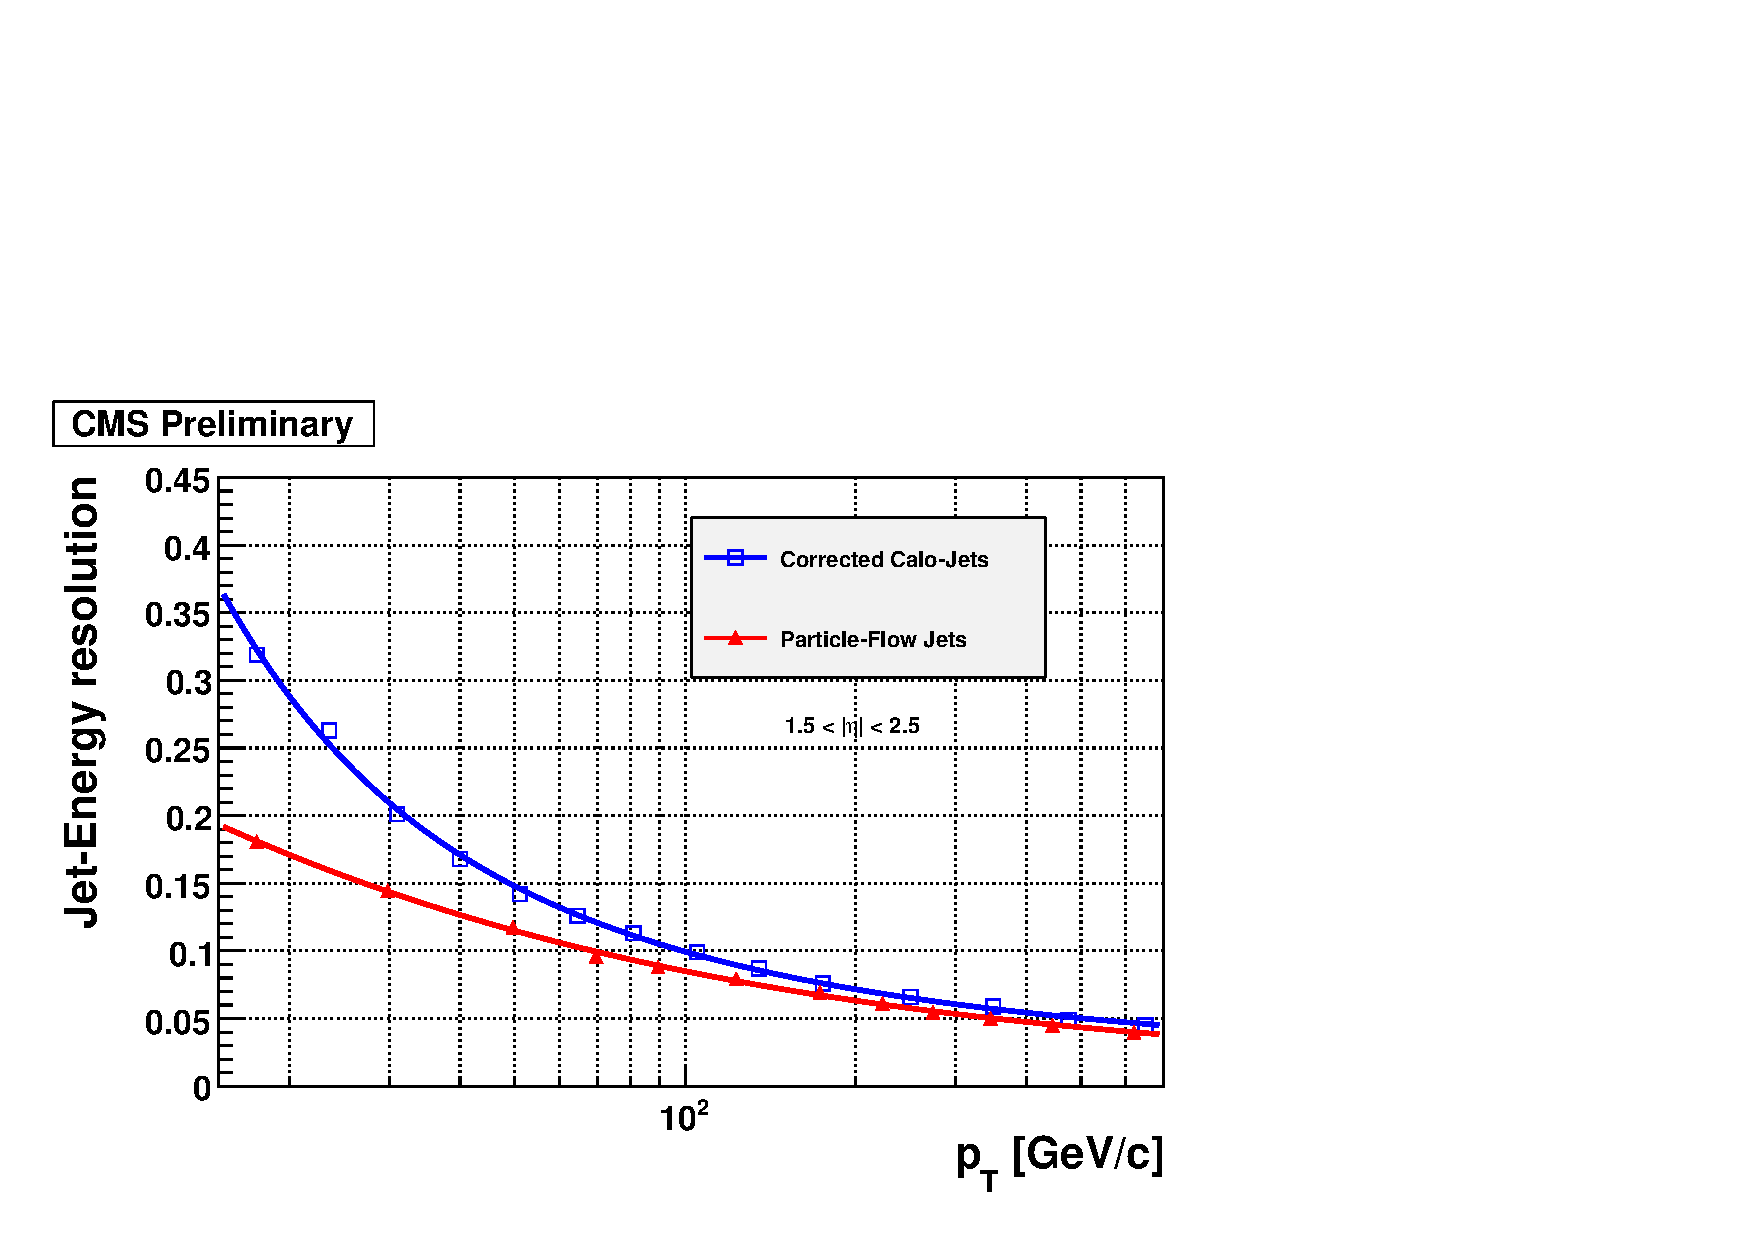
\includegraphics[width=0.45\textwidth]{fig/pf_jet_energyres_endcap}}\quad
\caption[Jet energy resolution as a function of \Pt]{Jet energy resolution as a
  function of \Pt for the \subref{fig:reco_pf_jet_energyres_barrel} barrel and
  \subref{fig:reco_pf_jet_energyres_endcap} endcap. Calo-jet values are
  displayed as open squares and \ac{PF} jet as upwards triangles. The curves are
  fit to the sum of a constant term, a stochastic term and a noise term.}
\label{fig:reco_pf_jet_energyres}
\end{figure}

\begin{figure}
\centering
\subfloat[]{\label{fig:reco_pf_jet_etares}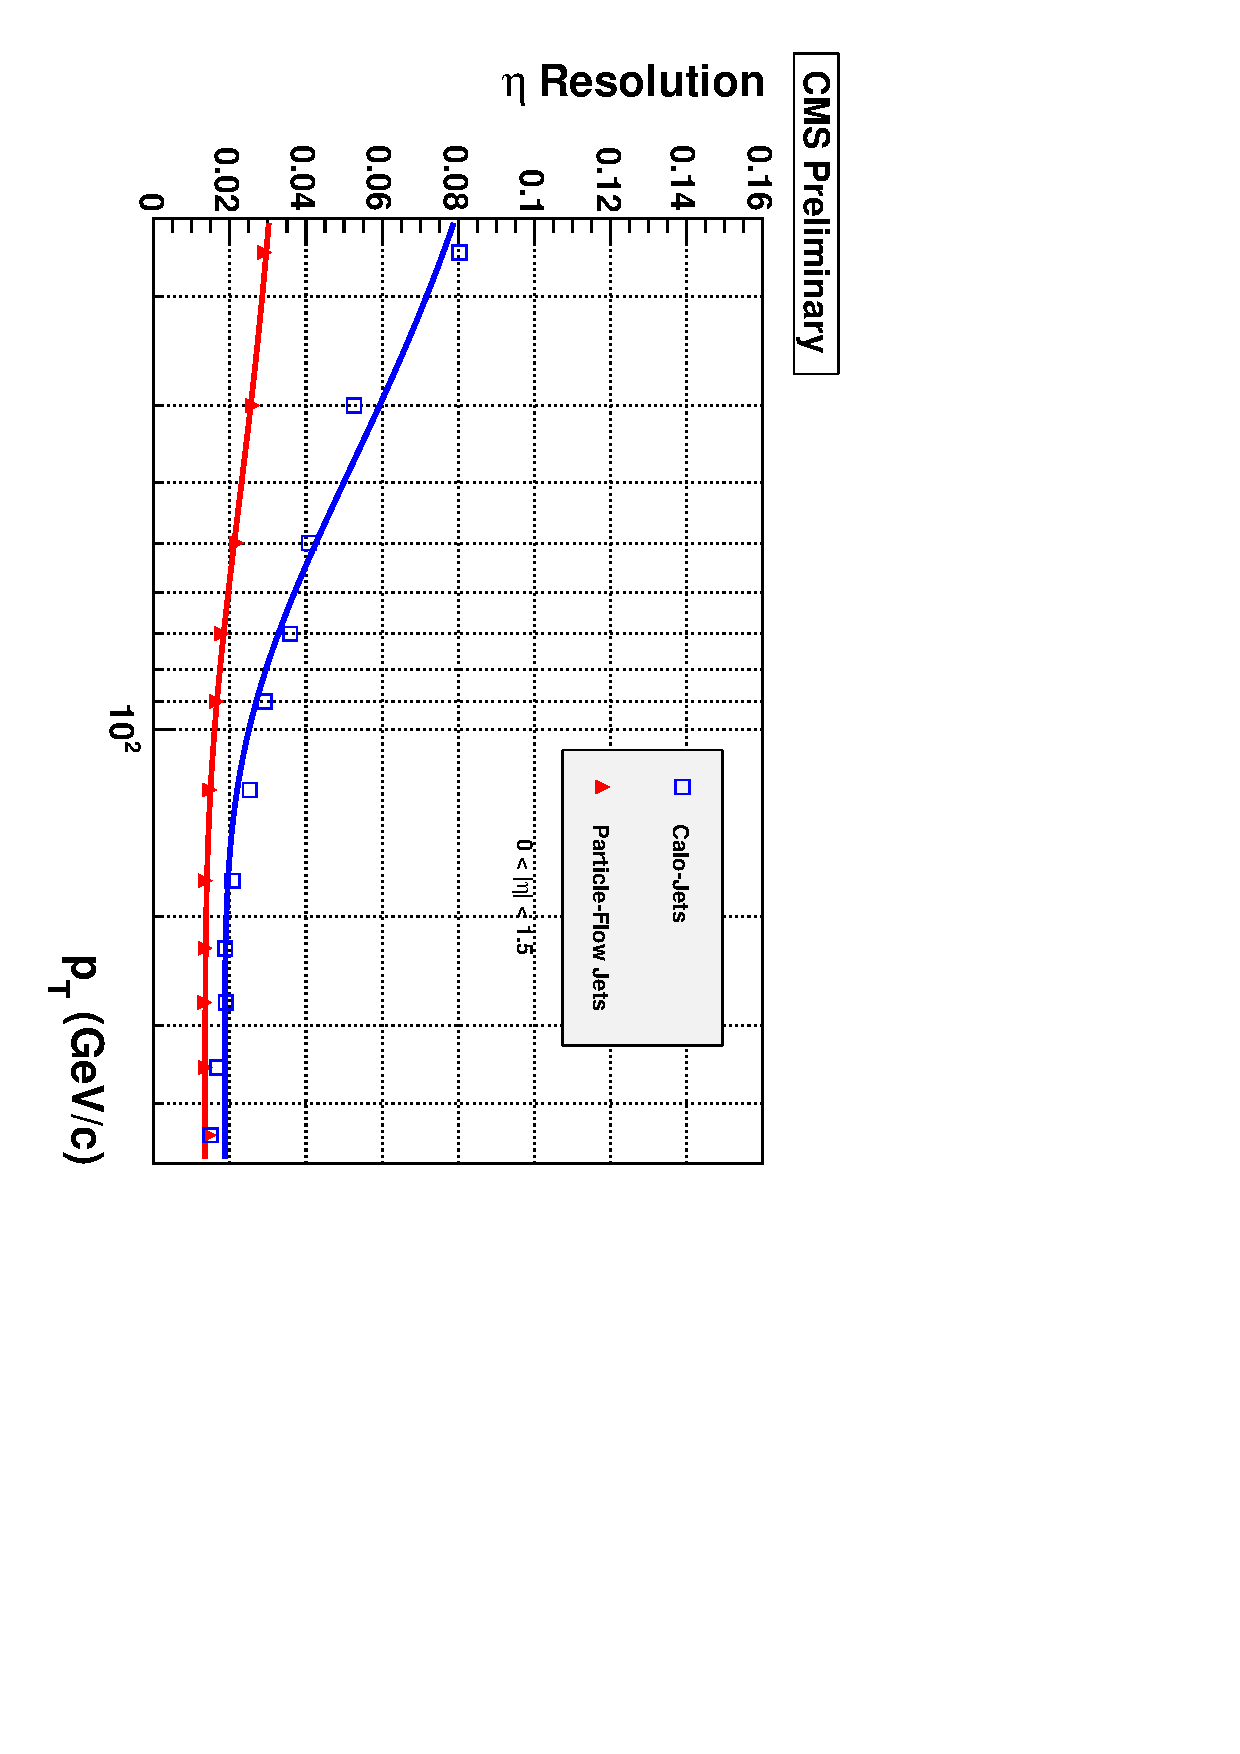
\includegraphics[width=0.45\textwidth]{fig/pf_jet_etares}}\quad
\subfloat[]{\label{fig:reco_pf_jet_phires}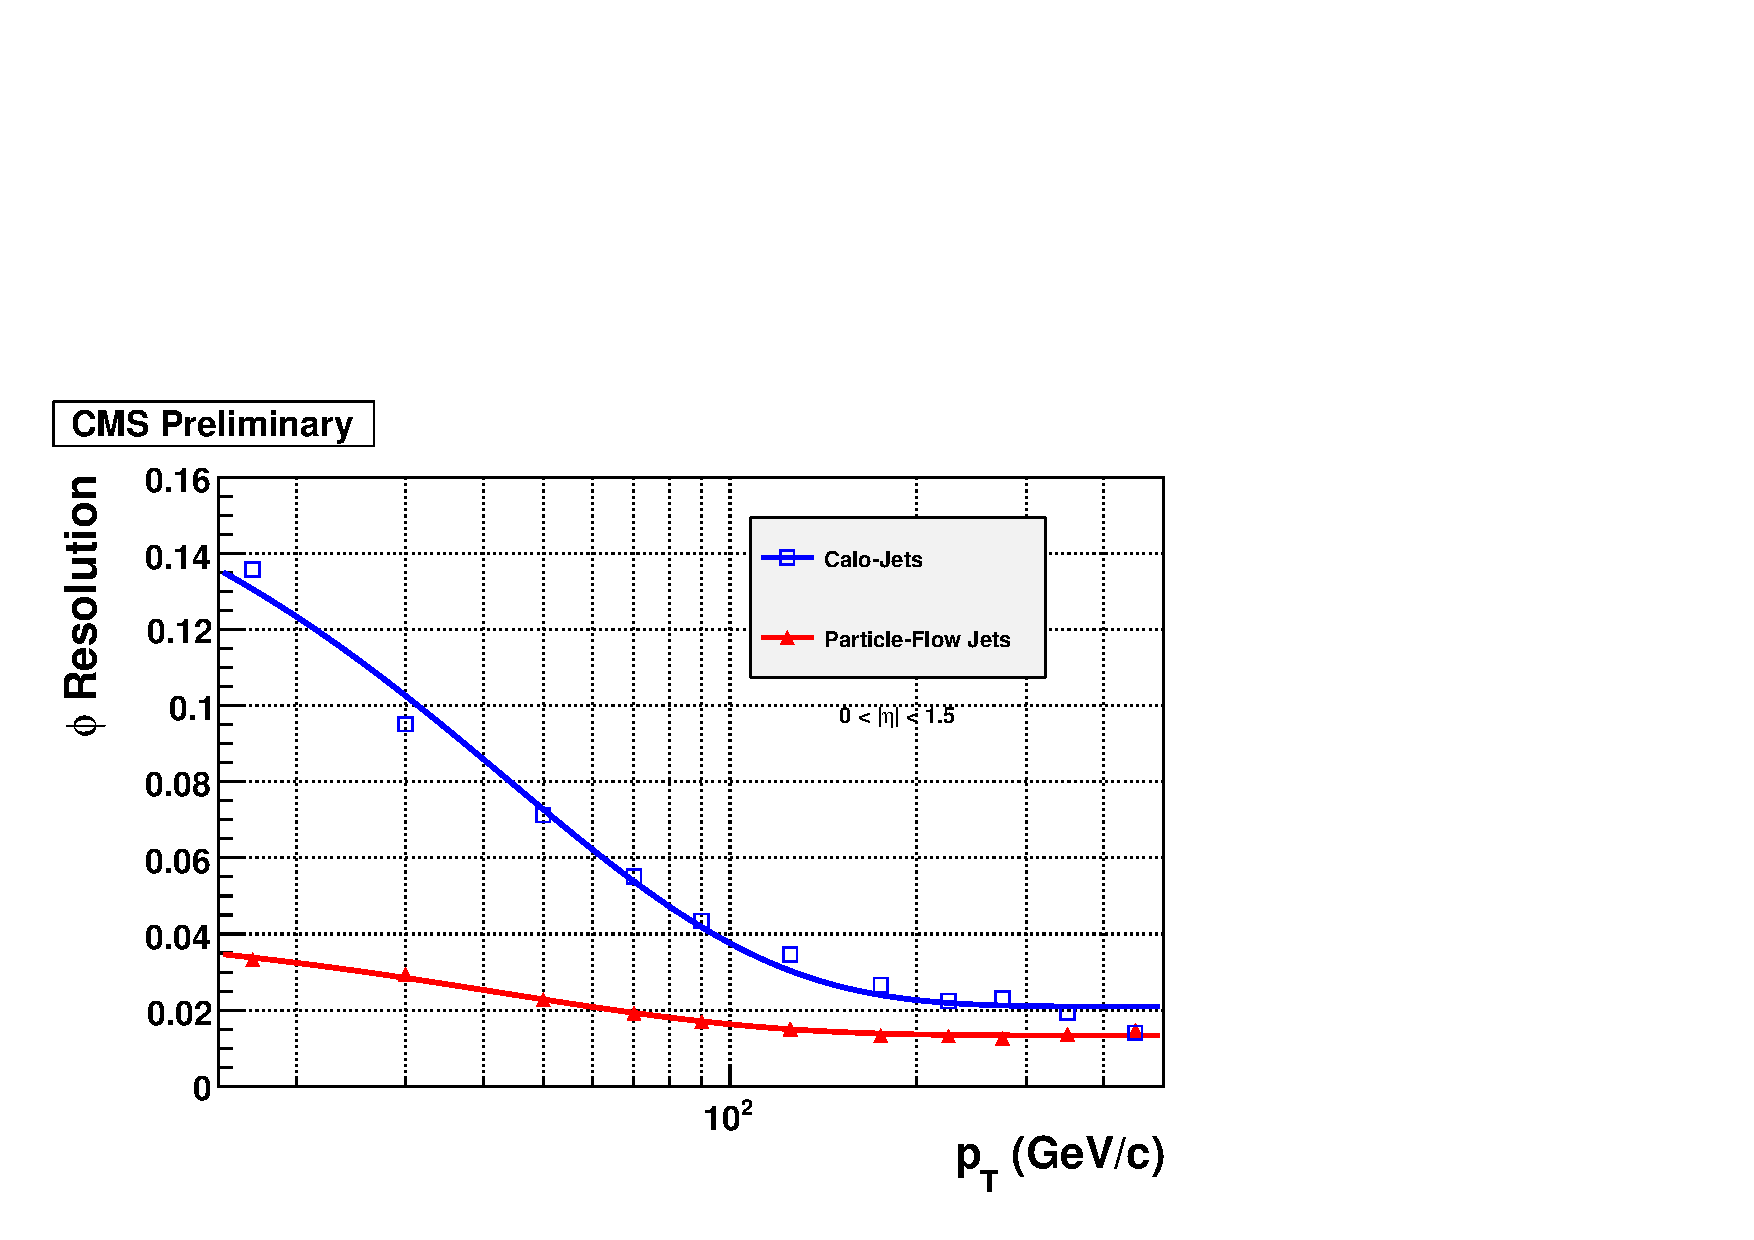
\includegraphics[width=0.45\textwidth]{fig/pf_jet_phires}}\quad
\caption[Jet angular resolution (\ac{RMS}) as a function of \Pt]{Jet angular
  resolution (\ac{RMS}) as a function of \Pt for \subref{fig:reco_pf_jet_etares}
  $\eta$ and \subref{fig:reco_pf_jet_phires} $\phi$. Calo-jets are shown as open
  squares and \ac{PF} jets as upward triangles. The curves are fit with an
  exponential function of $\Pt$.}
\label{fig:reco_pf_jet_angulares}
\end{figure}

\begin{figure}
\centering
\subfloat[]{\label{fig:reco_pf_met_metres}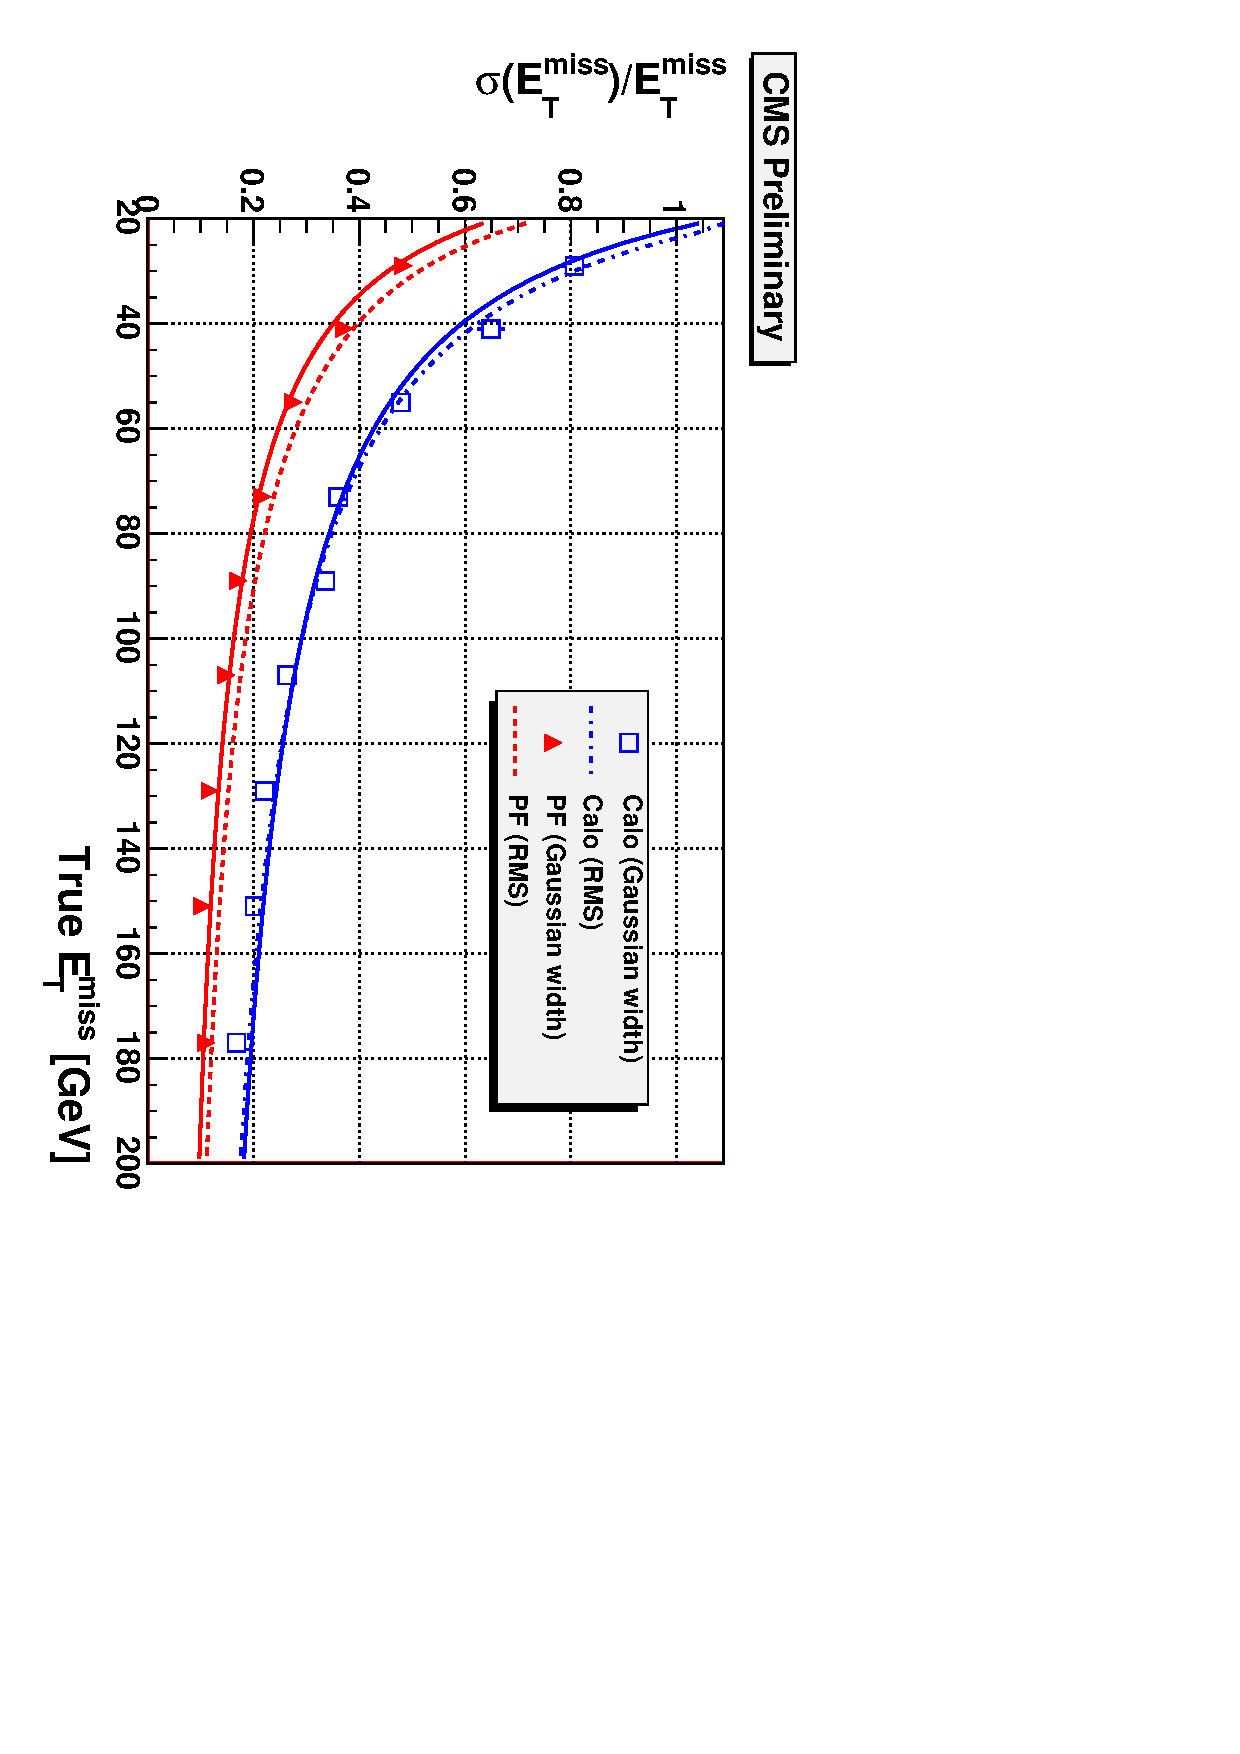
\includegraphics[width=0.45\textwidth]{fig/pf_met_metres}}\quad
\subfloat[]{\label{fig:reco_pf_met_phires}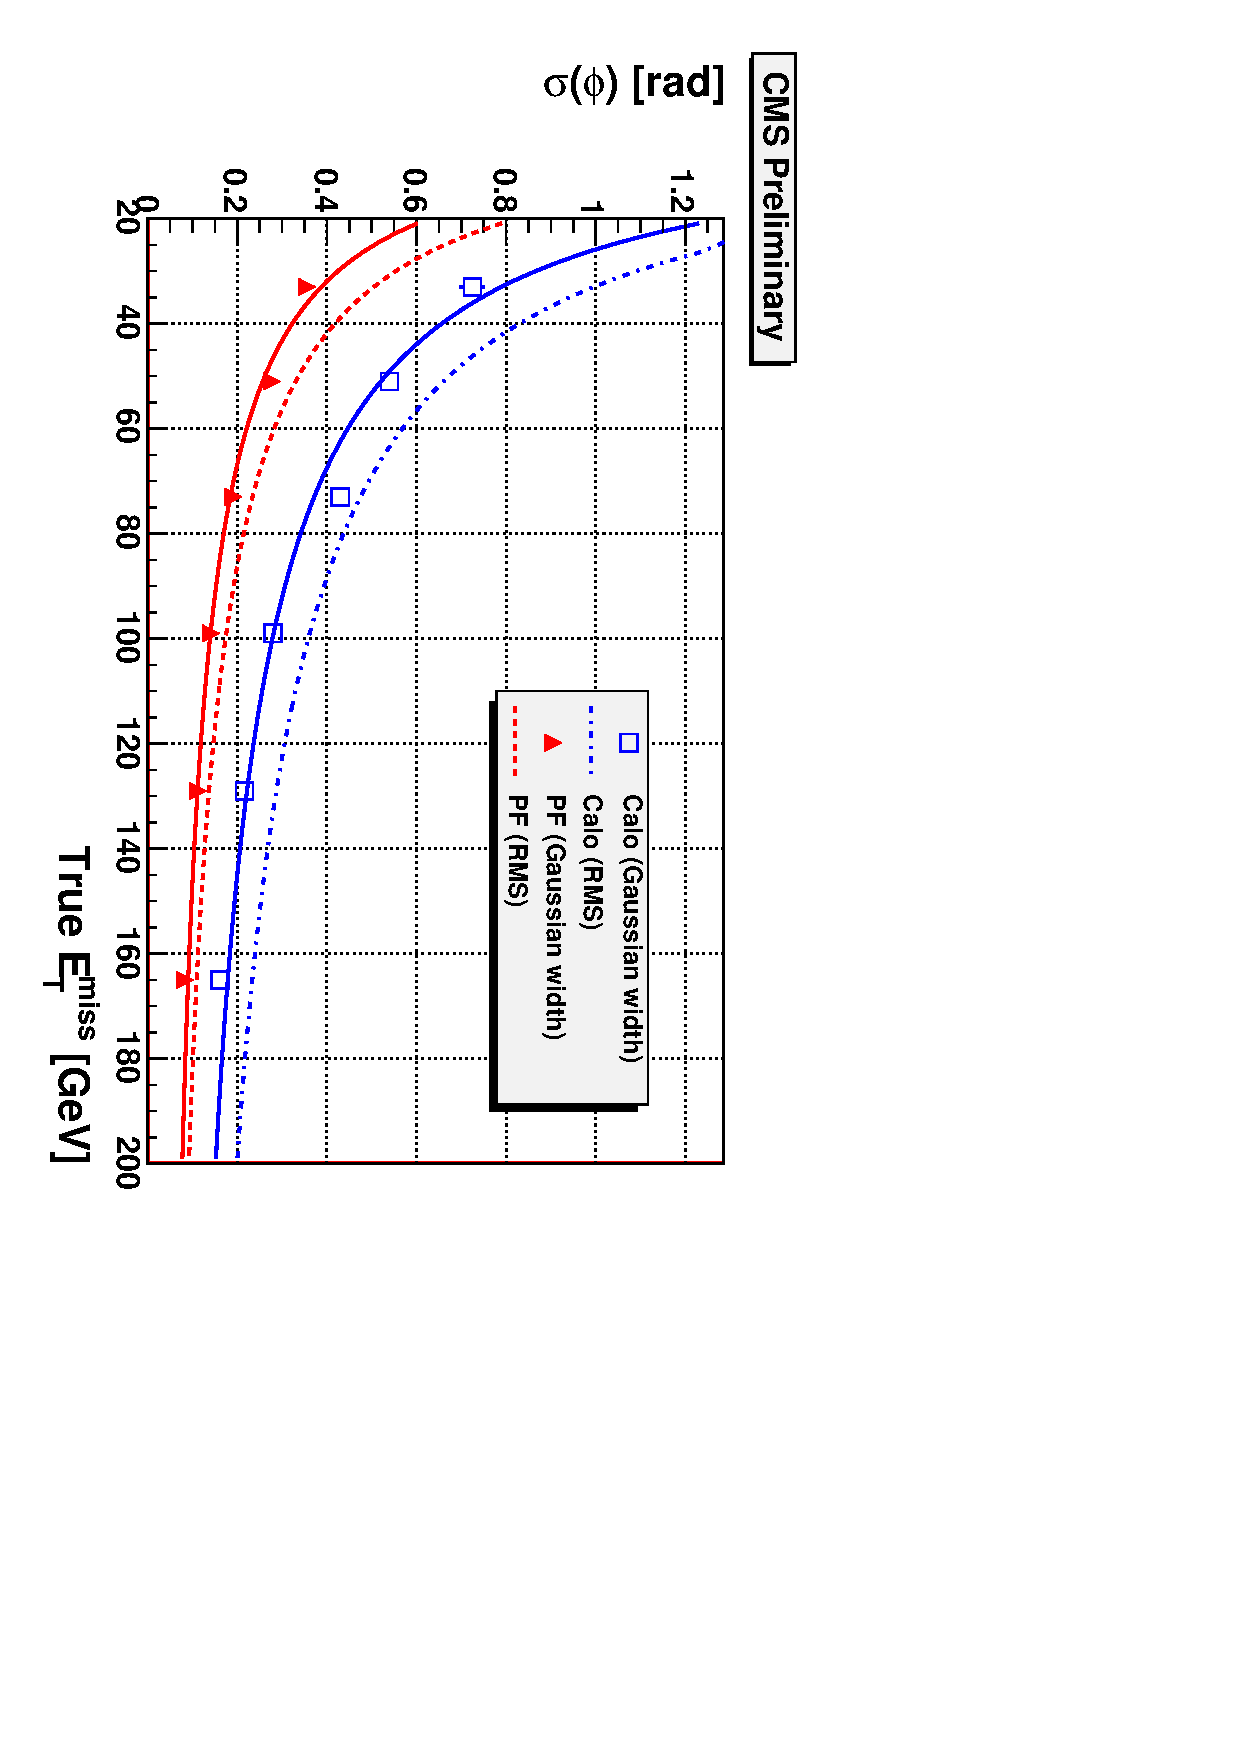
\includegraphics[width=0.45\textwidth]{fig/pf_met_phires}}\quad
\caption[\MET Resolution]{\subref{fig:reco_pf_met_metres}$\sigma(\MET)/\MET^{\textrm{true}}$ and
  \subref{fig:reco_pf_met_phires} $\sigma(\phi)$ as a function of true \MET in
  \ttbar events as determined by a Gaussian fit to each $\MET^{\textrm{true}}$
  bin. Squares represent Calo-\MET, and upwards triangles \ac{PF} \MET. The
  solid curves ares fits through these points. The dashed lines indicate the
  \ac{RMS} width of each bin.}
 \label{fig:reco_pf_met_res}
\end{figure}
